\documentclass[a4paper]{IEEEtran}
\pagestyle{empty}

\usepackage{graphicx}
\usepackage{url}
\usepackage[top=2.4cm,left=1.5cm,right=1.5cm,bottom=3.5cm]{geometry}
\usepackage{listings}
\usepackage{amssymb}

\setlength{\columnsep}{0.24in}
\setlength{\headsep}{0in}
\setlength{\parindent}{1.2pc}

\begin{document}

\title{Electromagnetic Characterisation of a Short-Stroke Ferromagnetic Actuator}
\author{R. M. Inston and H. Karimjee}

\maketitle
\begin{abstract}
This experiment demonstrated the use of FEMM as an analysis tool for a short stroke ferromagnetic actuator. 
\end{abstract}

\section{Nomenclature}
\begin{itemize}
\item[]{$R_{w}$, Winding resistance, [$\Omega$]}
\item[]{$l_{w}$, Length into the page of winding, [m]}
\item[]{$A_{w}$, Area of winding, [m$^{2}$]}
\item[]{$V_{w}$, Volume of winding, [m$^{3}$]}
\item[]{$N$, Number of turns in the winding, [-]}
\item[]{$\sigma$, Conductivity of winding, [Sm$^{-1}$]}
\item[]{$k_{PF}$, Packing factor of conductors in the winding, [-]}
\item[]{$L$, Inductance of the winding, [H]}
\item[]{$\mathcal{R}$, Reluctance, [H$^{-1}$]}
\item[]{$A_{eff}$, Effective area of air gap, [m$^{2}$]}
\item[]{$W$, Width of air gap, [m]}
\item[]{$T$, Thickness of air gap, [m]}
\item[]{$g$, Air gap length, [m]}
\end{itemize}

\section{Introduction}
% COULD PROBABLY DO WITH BULKING UP A BIT

Finite Element Method Magnetics (FEMM) is a subset of Finite Element Analysis (FEA) that specialises in electromagnetics. This tool, in combination with MatLab, can be used to program a series of analytical situations, from which the mechanical aspects of the system can be characterised. The actuator and core of the system share the same ferromagnetic properties, windings cover the top and bottom of the core and three air gaps of note exist, see figure \ref{xsection}.

\begin{figure}[ht]
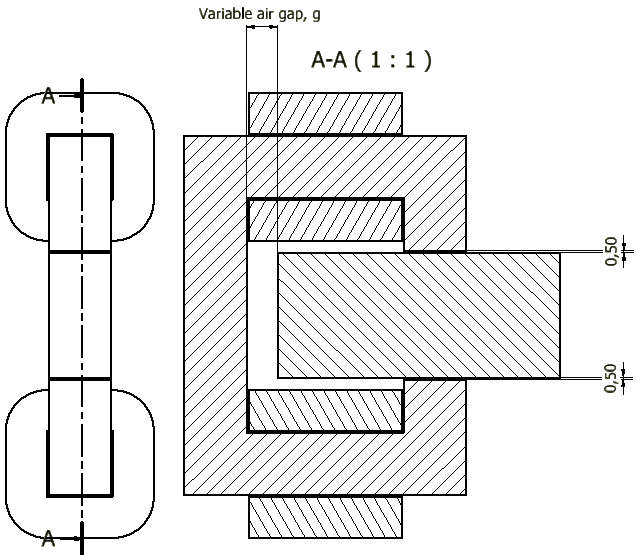
\includegraphics[width = \linewidth]{actuator-2.jpg}
\caption{Cross-sectional view of the actuator with the three air gaps higlighted (All measurements in mm).}
\label{xsection} 
\end{figure}

\section{Model Meshing}
To perform FEA, a model is split into elements. The elements must be small enough to output an accurate enough answer despite the linearisation of the physics occuring. Conversely, the elements cannot be too small as otherwise the computational time increases to an unfeasible (or uneconomical) amount.

FEMM has a smart-meshing tool in which the software analyses the model and allocates a dense mesh where the analysis must be of higher resolution and a sparse mesh where it does not. This is evident in figures \ref{noSmartMesh} \& \ref{smartMesh}. Although useful, this feature increases the mesh elements (see table \ref{meshTable}) and it does not know any information about the overarching complexity of the problem. One example of this is the boundaries involved with moving armature. Smart-meshing fails to recognise these edges as paramount to the analysis and produces a grid seen in figure \ref{zoomNotDense}. By manually increasing the density of meshing along these lines, FEMM can produce a more functional mesh seen in figure \ref{zoomDense}. This accuracy has its cost in terms of mesh elements and thus computational time, as seen in table \ref{meshTable}.

\begin{figure}[ht]
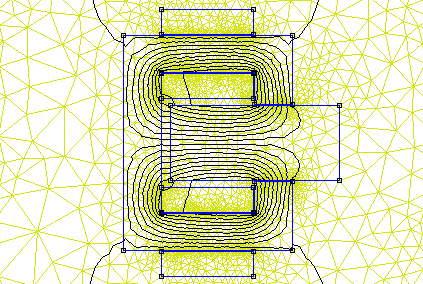
\includegraphics[width = \linewidth]{Smartmesh-OFF-NotDenseAirgap.png}
\caption{Example mesh with smart-meshing disabled. Note the sparseness of the triangulation.}
\label{noSmartMesh} 
\end{figure}

\begin{figure}[ht]
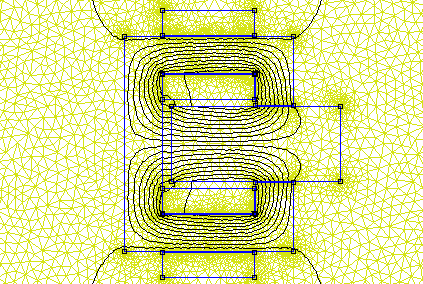
\includegraphics[width = \linewidth]{Smartmesh-ON-NotDenseAirgap.png}
\caption{Example mesh with smart meshing enabled. Note how the density increases around boundaries of interest.}
\label{smartMesh} 
\end{figure}

\begin{figure}[ht]
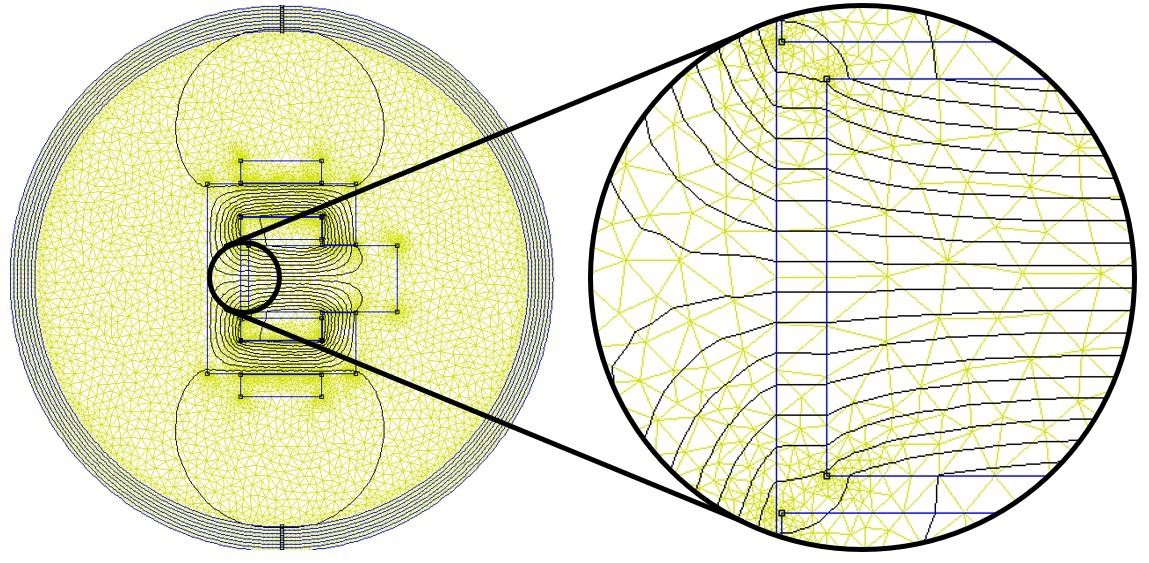
\includegraphics[width = \linewidth]{figurezoomnotdense.jpg}
\caption{FEMM smart-meshing output without specifying the area of interest. The density is low despite smart-meshing being on.}
\label{zoomNotDense} 
\end{figure}

\begin{figure}[ht]
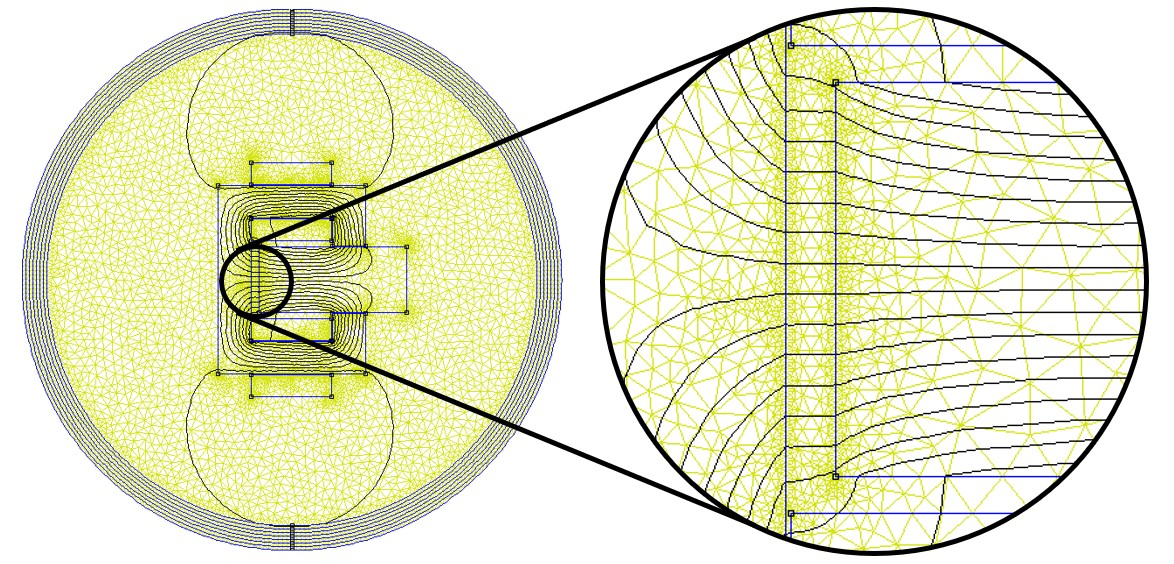
\includegraphics[width = \linewidth]{figurezoomdense.jpg}
\caption{FEMM smart-meshing output with specifying the area of interest and increasing the density of mesh elements within.}
\label{zoomDense} 
\end{figure}

\begin{table}[ht]
\centering
\begin{tabular}{ccc}
\textbf{\begin{tabular}[c]{@{}c@{}}Smart-\\ meshing\end{tabular}} & \textbf{\begin{tabular}[c]{@{}c@{}}Dense\\ Air gap\end{tabular}} & \textbf{\begin{tabular}[c]{@{}c@{}}Mesh\\ Elements\end{tabular}} \\ \hline
\multicolumn{1}{l}{} & \multicolumn{1}{l}{} & \multicolumn{1}{l}{} \\
OFF & OFF & 14790 \\
OFF & ON & 16334 \\
ON & OFF & 22668 \\
ON & ON & 24368 \\
\multicolumn{1}{l}{} & \multicolumn{1}{l}{} & \multicolumn{1}{l}{}
\end{tabular}
\caption{A summary of meshing options for the model.}
\label{meshTable}
\end{table}


\section{Winding Resistance}
To calculate the winding resistance, $R_{w}$, two approaches were used: FEMM and analytical. FEMM can calculate the winding's resistance by getting the circuit properties of each winding and obtaining the voltage and current. The analytical approach used block integrals in FEMM to obtain volume and area of the winding and hence the depth into the page can be found using equation \ref{length}:

\begin{equation}
l_{w} = \frac{V_{w}}{A_{w}}
\label{length}
\end{equation}

The resistance is thus calculated using equation \ref{resistance}. The resistances of each calculation method are presented in table \ref{windingResistance}. 

\begin{equation}
R_{w} = \frac{N l_{w}}{\sigma\left(\frac{k_{PF} A_{w}}{N}\right)}
\label{resistance}
\end{equation}

Notable in table \ref{windingResistance} is the difference in estimated values. The analytical value uses the packing factor, $k_{PF}$, that compensates for the space used by the insulating material in a winding. FEMM sees the entire area as conducting material and hence the implied length of wire increases. Given the conductivity, $\sigma$, is the same in both predictions; the greater the implied length of winding, the greater the winding resistance, $R_{w}$. However, FEMM is working with a 2D model and the analysis was performed on the top section of the winding only. This means the analysis does not account for the mean path length around the winding, causing the FEMM estimate to be at least a factor of four out from the analytical prediction. 

\begin{table}[ht]
\centering
\begin{tabular}{c|cc}
\textbf{Method} & \textbf{Current {[}A{]}} & \textbf{\begin{tabular}[c]{@{}c@{}}Winding\\ Resistance {[}$\Omega${]}\end{tabular}} \\ \hline
 &  &  \\
FEMM & 10 & 0.0107 \\
Analytical & 10 & 0.0557
\end{tabular}
\caption{A summary of winding resistance calculation for different methods.}
\label{windingResistance}
\end{table}

These two methods were plotted for many values of current and the power loss of the winding calculated. The resulting graph can be seen in figure \ref{windingLoss}.

\begin{figure}[ht]
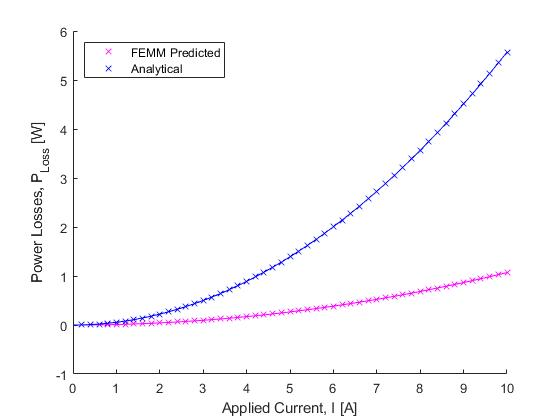
\includegraphics[width = \linewidth]{ResistanceWindingLoss.jpg}
\caption{Power loss against current shown for the FEMM predicted values and Analytical evaluation. A quadratic curve produces the line of best fit.}
\label{windingLoss} 
\end{figure}

\section{Winding Inductance}
The inductance of the windings can be found analytically and numerically. To estimate the value analytically, equation \ref{inductance} is followed. 

\begin{equation}
L = \frac{N^2}{\sum{\mathcal{R}}}
\label{inductance}
\end{equation}

To find an analytical expression for the inductance where flux is assumed to be conserved:
\begin{equation}
\mathcal{R} =  \frac{l}{\mu_{0}\mu_{r}A}
\label{reluctance}
\end{equation}


\begin{equation}
\sum{\mathcal{R}} = \mathcal{R}_{core} + \mathcal{R}_{air} + \mathcal{R}_{armature} + \mathcal{R}_{gap}
\label{summm}
\end{equation}

Or fringing effects can be taken into account by substituting equation \ref{EffectiveArea} into equation \ref{reluctance} for $\mathcal{R}_{gap}$ and $\mathcal{R}_{air}$. 

\begin{equation}
A_{eff} = (W + 2g)(T + 2g)
\label{EffectiveArea}
\end{equation}

This gives a total of two analytical values. Numerically, two values of inductance can be estimated using FEMM by using a linear or non-linear approximation of core and armature properties. The inductance varies with the displacement of the armature, evident in figure \ref{inductanceGraph}.

\begin{figure}[ht]
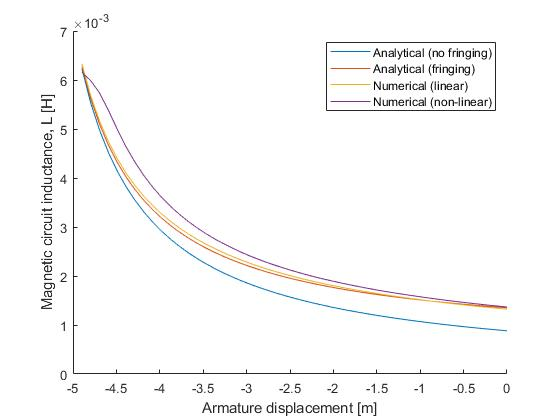
\includegraphics[width = \linewidth]{Inductances.jpg}
\caption{Graph showing inductance versus armature displacement for the varying methods of calculation.}
\label{inductanceGraph} 
\end{figure}


\section{Force on the Armature}
% NEEDS A CHEEKY WRITE UP



\begin{figure}[ht]
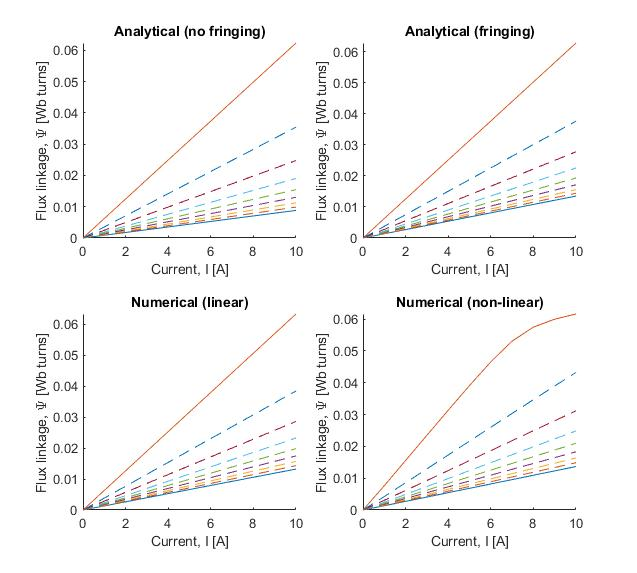
\includegraphics[width = \linewidth]{psi-I-diagrams.jpg}
\caption{$\Psi$-I diagrams for the four methods of calculating inductance. Note the saturation visible in the non-linear graph. Shown for zero displacement, maximum displacement ($-49$mm) and seven linearly spaced intervals between (shown as the dashed lines).}
\label{psi-eye} 
\end{figure}

\begin{figure}[ht]
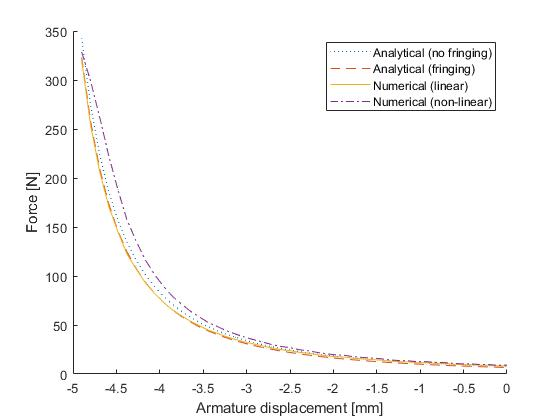
\includegraphics[width = \linewidth]{Force-Displacement.jpg}
\caption{Force versus displacement for the four methods of calculating inductance. Tabulated values evident in table \ref{coenergy}.}
\label{forceGraph} 
\end{figure}

\begin{table}[]
\centering
\begin{tabular}{c|cccc}
 & \multicolumn{4}{c}{\textbf{Change in Co-Energy {[}J{]}}} \\
\textbf{\begin{tabular}[c]{@{}c@{}}Armature\\Displacement\\{[}mm{]}\end{tabular}} & \textbf{\begin{tabular}[c]{@{}c@{}}Analytical\\(no\\fringing)\end{tabular}} & \textbf{\begin{tabular}[c]{@{}c@{}}Analytical\\(fringing)\end{tabular}} & \textbf{\begin{tabular}[c]{@{}c@{}}Numerical\\(linear)\end{tabular}} & \textbf{\begin{tabular}[c]{@{}c@{}}Numerical\\(non-\\linear)\end{tabular}} \\ \hline
0.200 & 7.867 & 6.620 & 8.442 & 9.110 \\
0.300 & 8.158 & 6.888 & 8.264 & 8.826 \\
0.400 & 8.467 & 7.172 & 8.930 & 9.635 \\
0.500 & 8.793 & 7.473 & 8.977 & 9.694 \\
0.600 & 9.138 & 7.791 & 9.511 & 10.27 \\
0.700 & 9.505 & 8.128 & 9.589 & 10.33 \\
0.800 & 9.893 & 8.486 & 10.09 & 10.93 \\
0.900 & 10.31 & 8.867 & 10.74 & 11.68 \\
1.000 & 10.75 & 9.272 & 10.91 & 11.83 \\
1.100 & 11.21 & 9.703 & 11.67 & 12.68 \\
1.200 & 11.71 & 10.16 & 11.64 & 12.64 \\
1.300 & 12.25 & 10.66 & 12.39 & 13.55 \\
1.400 & 12.82 & 11.18 & 12.58 & 13.72 \\
1.500 & 13.43 & 11.75 & 13.20 & 14.43 \\
1.600 & 14.09 & 12.35 & 14.20 & 15.62 \\
1.700 & 14.79 & 13.00 & 14.82 & 16.31 \\
1.800 & 15.55 & 13.71 & 15.34 & 16.87 \\
1.900 & 16.37 & 14.46 & 16.03 & 17.72 \\
2.000 & 17.26 & 15.28 & 17.30 & 19.13 \\
2.100 & 18.22 & 16.17 & 17.62 & 19.60 \\
2.200 & 19.26 & 17.14 & 18.63 & 20.66 \\
2.300 & 20.40 & 18.19 & 19.74 & 22.06 \\
2.400 & 21.64 & 19.33 & 21.20 & 23.68 \\
2.500 & 23.00 & 20.59 & 22.11 & 24.81 \\
2.600 & 24.48 & 21.97 & 23.88 & 26.92 \\
2.700 & 26.12 & 23.48 & 24.86 & 28.09 \\
2.800 & 27.93 & 25.16 & 26.49 & 29.95 \\
2.900 & 29.93 & 27.01 & 28.66 & 32.69 \\
3.000 & 32.15 & 29.07 & 30.61 & 34.99 \\
3.100 & 34.64 & 31.38 & 32.77 & 37.65 \\
3.200 & 37.42 & 33.96 & 35.27 & 40.75 \\
3.300 & 40.55 & 36.87 & 38.03 & 44.09 \\
3.400 & 44.09 & 40.16 & 41.48 & 48.39 \\
3.500 & 48.11 & 43.9 & 44.66 & 52.40 \\
3.600 & 52.71 & 48.19 & 49.25 & 58.24 \\
3.700 & 58.01 & 53.12 & 53.90 & 64.19 \\
3.800 & 64.14 & 58.85 & 59.57 & 71.51 \\
3.900 & 71.3 & 65.54 & 65.68 & 79.57 \\
4.000 & 79.74 & 73.42 & 73.48 & 89.84 \\
4.100 & 89.76 & 82.81 & 82.65 & 102.2 \\
4.200 & 101.8 & 94.10 & 93.52 & 116.9 \\
4.300 & 116.4 & 107.9 & 107.3 & 136.0 \\
4.400 & 134.5 & 124.8 & 122.6 & 157.4 \\
4.500 & 157.0 & 146.1 & 145.1 & 188.2 \\
4.600 & 185.8 & 173.4 & 170.7 & 222.4 \\
4.700 & 223.3 & 209.0 & 206.0 & 261.7 \\
4.800 & 273.5 & 256.8 & 253.1 & 298.5 \\
4.900 & 342.6 & 323.0 & 319.8 & 328.5
\end{tabular}
\caption{Tabulated data for the change in co-energy for all changes in position, given to 4 significant figures.}
\label{coenergy}
\end{table}


\section{Conclusion}
% NEEDS FINALISING


\pagebreak
\onecolumn
\section{Appendix}
\textsc{\textbf{The following is a listing of the Matlab script written to construct the actuator:}}
\lstinputlisting[language=Matlab]{construct_actuator_copy.m}

\pagebreak
\textsc{\textbf{The following is a listing of the Matlab script written to analyse the actuator:}}
\lstinputlisting[language=Matlab]{analyse_actuator_copy.m}
 
\pagebreak
\textsc{\textbf{The following is a listing of the Matlab script written to produce the graphs and tables:}}
\lstinputlisting[language=Matlab]{process_copy.m}


\end{document}